
% !TeX spellcheck = de_DE
\documentclass{article}

\usepackage[ngerman]{babel}
\usepackage{graphicx}
\usepackage{indentfirst}
\usepackage{hyperref}
\usepackage{geometry}
\usepackage{changepage}
\usepackage{booktabs}
\usepackage{float}
\usepackage{tabulary}
\usepackage{multirow}

\graphicspath{ {./images/} }

\makeatletter
\newcommand{\sectionauthor}[1]{
	{\parindent 0em \large \scshape Autor: #1 \par \nobreak \vspace*{1em}}
	\@afterheading
}
\newcommand{\specification}[3]{
	{\parindent 0.5em \hangindent 3em \hypertarget{spec:#1:#2}{\textbf{/#1#2/}} #3 \par \nobreak \vspace*{0.5em}}
}
\makeatother

\begin{document}

%--Einleitung--------------------------------------------------------------------------------------------------------------------------------------------------------------------------
\section{Einleitung}
\sectionauthor{Jonas Picker}
Hier wird der Entwurf des Bibliotheksmanagementsystems BiBi beschrieben. Das Dokument bezieht sich auf das Lastenheft von Christian Bachmaier und Armin Größlinger und stellt eine technische Vertiefung unseres Pflichtenhefts dar, welches im Folgenden wiederholt referenziert wird.

%--Systemarchitektur---------------------------------------------------------------------------------------------------------------------------------------------------------------
\section{Systemarchitektur}
\sectionauthor{Ivan Charviakou}

\subsection{Design-Patterns: Schichtenunabhängigkeit}

MVC: Als grundlegendes Design-Pattern sorgt MVC dafür, dass die Model-, Präsentations-, und Steuerungskomponente voneinander weitgehend entkoppelt sind. Dabei implementiert das JSF-Framework per Default Großteile der Präsentations- und Steuerungskomponenten, aber überlässt die Modelkomponente komplett dem Entwickler. Für die Präsentationskomponente werden nämlich vordefinierte UI-Komponente vorgesehen, während der eingebaute Faces-Servlet die Steuerungsaufgabe übernimmt. Durch selbst-definierte Tag-Libraries und Facelets lassen sich diese beiden Komponenten auch ggf. vervollständigen. \vspace{0.5em}

CDI: Die im JSF-Framework eingebaute CDI-Funktionalität ermöglicht eine direkte Kommunikation zwischen abhängigen Komponenten, die durch JSF verwaltet werden. Solche Beziehungen werden dann mit entsprechenden Annotationen, wie ‚@inject‘, gekennzeichnet. In der gegebenen Anwendung trägt CDI dadurch wesentlich zur Intraschichtenkommunikation bei. \vspace{0.5em}

DTOs: Ein Datentransferobjekt (DTO) enthält die Daten zu einer bestimmten Entität oder zu einem zusammenhängenden Ausschnitt aus verschiedenen Entitäten. In der gegebenen Anwendung entspricht das einem Medium, Exemplar, Nutzer, usw. Durch Übergabe von solchen Objekten an verschiedenen Modelschichten, können sie die Daten unabhängig voneinander anpassen oder evaluieren. Als Beispiel prüft im Model die Logikschicht das Format eines E-Mails, während die Sicherheitsschicht SQL-Injection-Attacken in der Eingabe ausschließt. \vspace{0.5em}

DAOs und ihre Fassaden: Zu jedem DTO existiert auch ein Datenzugriffsobjekt (DAO), das bei einer Übergabe eines DTOs die enthaltenen Daten speichert bzw. lädt. Damit mehrere Modelschichten diese Prozeduren eigens erweitern können, verwenden die DTOs in der gegebenen Anwendung den Fassade-Muster. Jede betroffene Schicht verwendet zur Erweiterung eines DAOs nämlich die gleiche Schnittstelle und ruft die Schnittstelle der nächsten Schicht auf. Als Beispiel gibt die Logikschicht ein Passwort im Klartext an und übergibt es an eine DAO-Instanz in der Sicherheitsschicht mittels eines DTOs. Diese Schicht berechnet dann aus dem Klartext einen Hash-Wert und leitet diesen Wert an die DAO-Instanz in der Datenzugriffsschicht weiter. \vspace{0.5em}

Event-Listener: Dadurch, dass JSF verschiedene Arten von Listenern bereitstellt, ist eine stärkere Entkopplung von Schichten möglich. Während Action-, Value-Change-, und Phasenlistener hauptsächlich eine Logikschicht ansprechen, kann beispielweise der eingebaute System-Event-Listener für die unabhängige Initialisierung der Modelschichten sorgen.

\subsection{Design-Patterns: Fehlerbehandlung}

Allgemeiner Testmodus: Es wird ein Testmodus eingeführt, der beim Applikationsstart als Parameter angegeben wird. \vspace{0.5em}

Exceptions: Jede Schicht in der gegebenen Anwendung definiert eigene Checked-Exceptions, die ggf. durch die Schichten hochgeworfen werden. Dabei wird eine solche Exception in jeder Zwischenschicht gefangen in eine eigens definierte Exception umgewandelt bis eine Schicht sie behandelt. Im Gegensatz werden Unchecked-Exceptions nicht behandelt und führen zum Absturz der Anwendung. Während für eine Präsentations- und Logikschicht oft eine GUI-Anzeige als geeignete Behandlung gilt, ist es für jede Schichten anders. Falls es beispielsweise durch eine Checked-Exception in der Datenzugriffsschicht festgestellt wird, dass die verwendete Datenbank nicht mehr erreichbar ist, wird stattdessen dynamisch auf lokale Applikationsdaten zugegriffen. Unter den DAOs in der Datenzugriffsschicht wird somit der Strategy-Muster angewendet. \vspace{0.5em}

Logging: Als Logging-Framework wird der im JDK vordefinierte Framework verwendet. Diese Funktionalität ist nur im Testmodus aktiv und es wird zu einer lokalen Log-Datei geschrieben. \vspace{0.5em}

Validatoren: Das JSF-Framework gibt dem Entwickler die Möglichkeit, Daten auf Korrektheit zu prüfen, bevor sie dem Logikschicht bereitgestellt wird. Da aber komplexere semantische Fehler oft einen größeren Kontext und eine komplexere Behandlung benötigen, wird der Einsatz von diesen Validatoren hauptsächlich auf syntaktische Formattierfehler beschränkt.

\subsection{Design-Patterns: Konkrete Features}

Connection-Pool: Unter einem Pool bezeichnet man eine Sammlung an Objekten, die angefragt, zurückgegeben, und wiederverwendet werden. Dies vermeidet insbesondere die Erzeugung von solchen Objekten, was in Bezug auf Datenbankverbindungen als aufwendig gilt. Da es trivialerweise nur einen solchen Container geben sollte, wird ein Pool auch als Singleton verwendet. Für die gegebene Anwendung wird die HikariCP Implementierung einer solchen Connection-Pool genommen. Beim Testmodus wird die Anzahl an Verbindungen auf eins gesetzt. \vspace{0.5em}

Wartungsthread: In der gegebenen Anwendung kann es vorkommen, dass persistierte Daten oder Daten im Cache mit der Zeit ungültig werden. Du solchen Daten gehört beispielsweise die Gültigkeit von einem Passwortrücksetzungslink. Mit einem Wartungsprozess werden solche Inkonsistenzen erkannt und behoben.

\subsection{Modeldiagramm}

\begin{figure}[H]
	\centering
	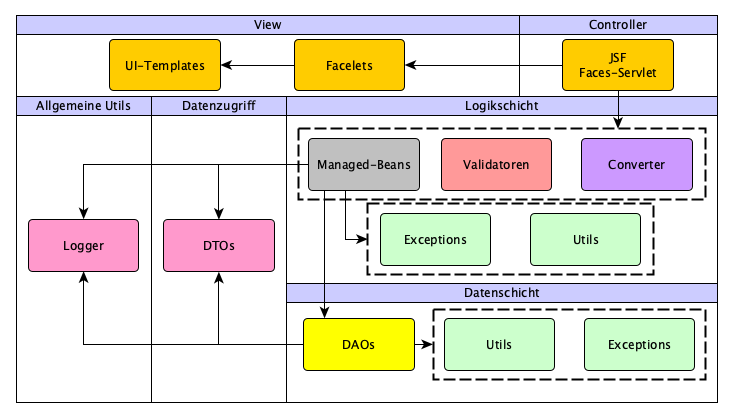
\includegraphics[width = 50em]{Modeldiagramm}
\end{figure}

%--Klassendiagramm---------------------------------------------------------------------------------------------------------------------------------------------------------------

\section{Klassendiagramm}
\sectionauthor{Mohamad Najjar}

%   \begin{landscape}
    \begin{figure}
        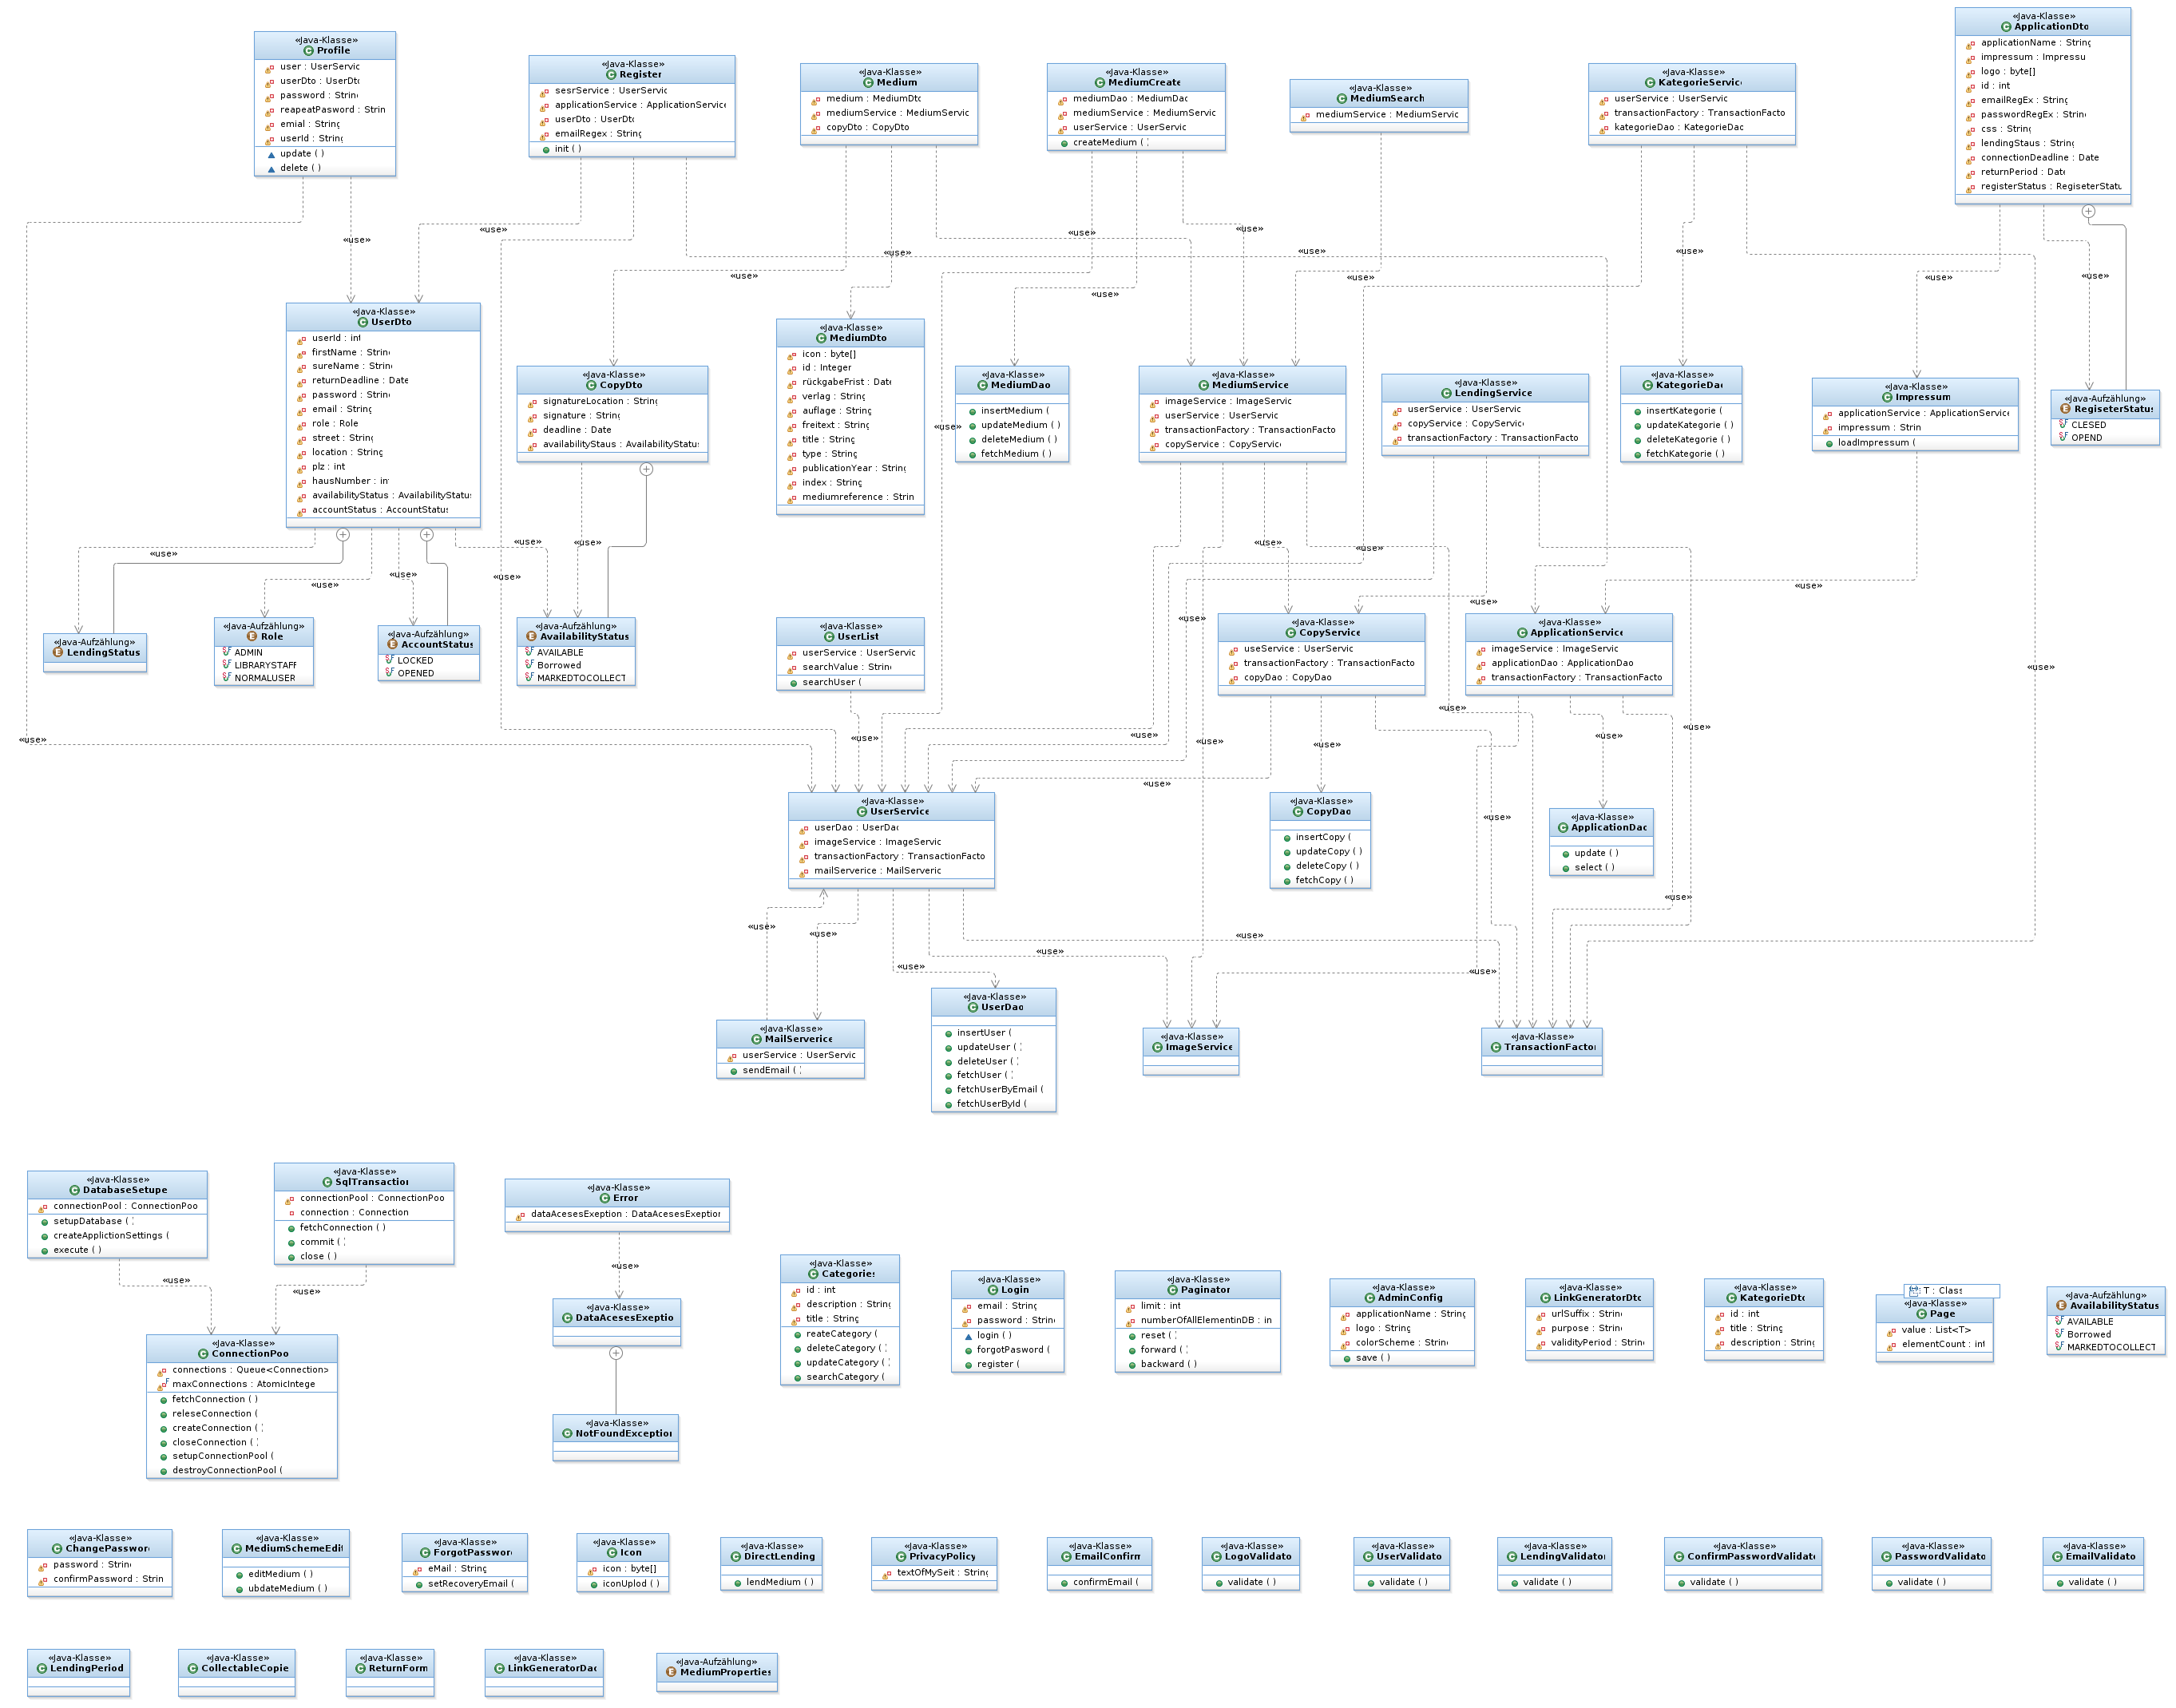
\includegraphics[scale=0.2]{Klassendiagramm.png}
        \caption{Klassendiagramm}
        \label{fig:Klassendiagramm}
    \end{figure}
%    \end{landscape}

%    \begin{landscape}
    \begin{figure}
        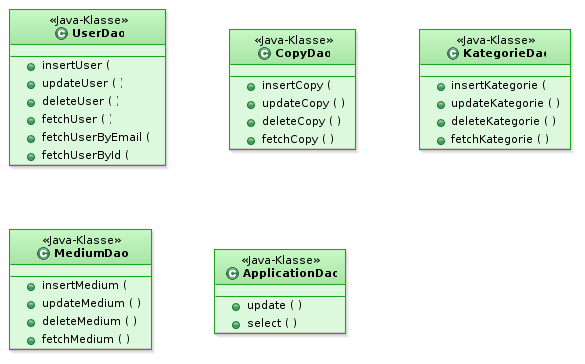
\includegraphics[scale=0.6]{KlassendiagramDao.png}
        \caption{Klassendiagramm der Daos}
        \label{fig:KlassendiagramDao}
    \end{figure}
%    \end{landscape}

%    \begin{landscape}
    \begin{figure}
    \centering
        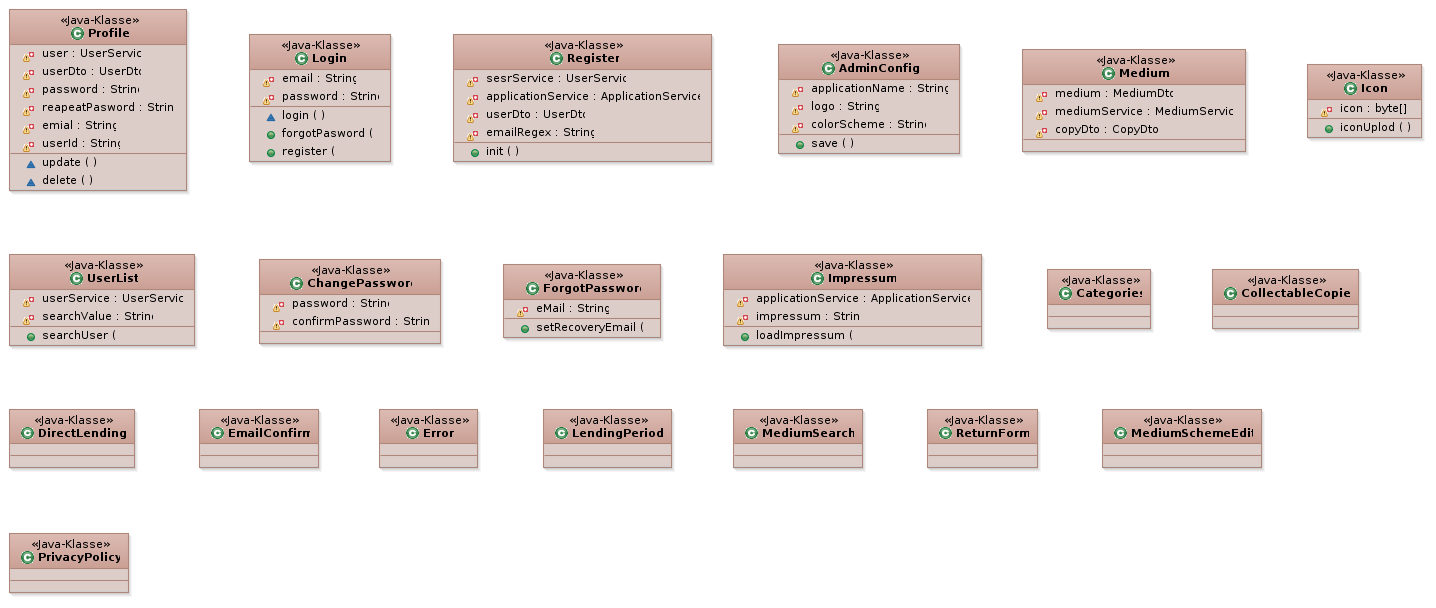
\includegraphics[scale=0.7, angle=270]{KlassendiagramBeans.png}
        \caption{Klassendiagramm der Beans}
        \label{fig:KlassendiagramBeans}
    \end{figure}
%    \end{landscape}

%    \begin{landscape}
    \begin{figure}
        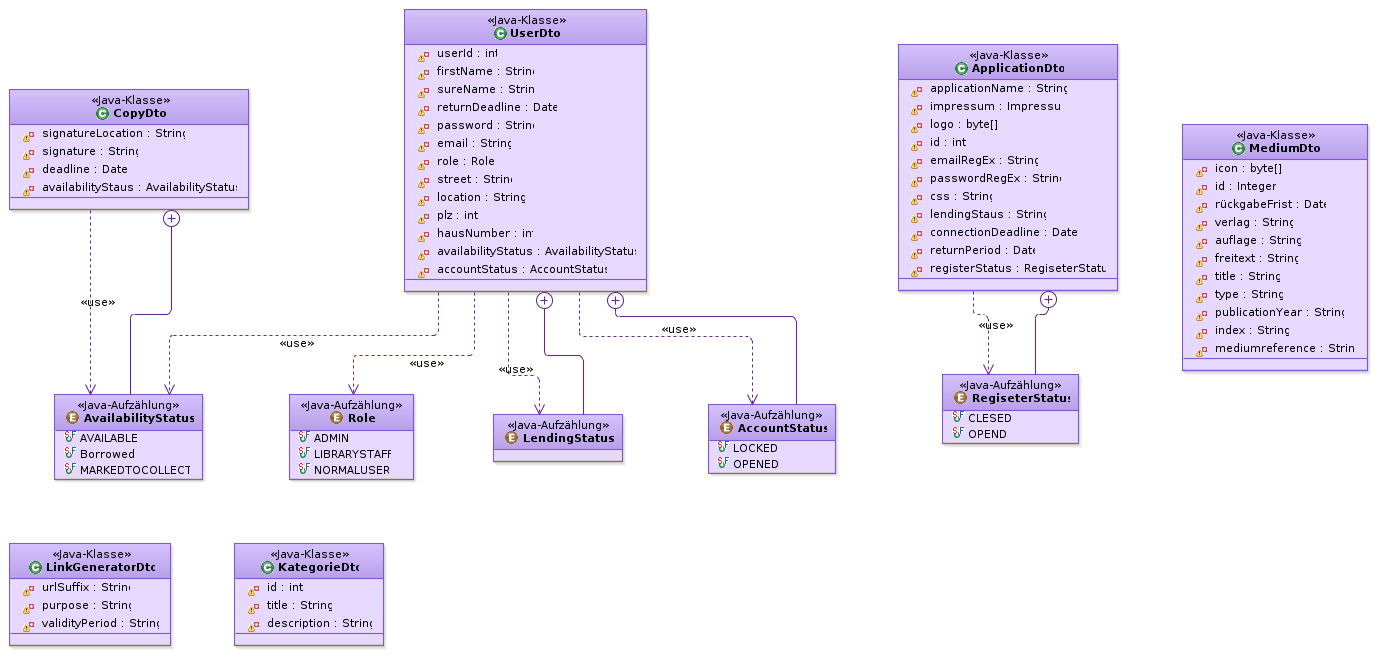
\includegraphics[scale=0.6]{KlassendiagramDtos.png}
        \caption{Klassendiagramm der Dtos}
        \label{fig:KlassendiagrammDto}
    \end{figure}
%    \end{landscape}


%    \begin{landscape}
    \begin{figure}
        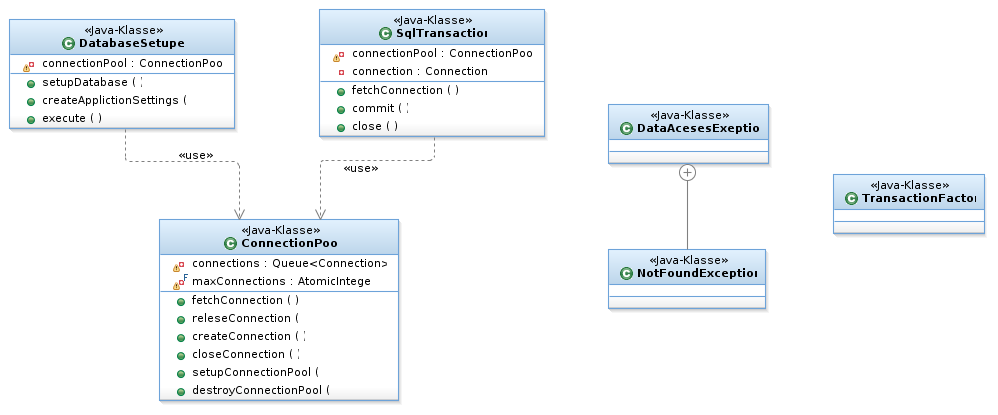
\includegraphics[scale=0.6]{KlassendiagramSystem.png}
        \caption{Klassendiagramm des Systems}
        \label{fig:KlassendiagramSystem}
    \end{figure}
%    \end{landscape}

%    \begin{landscape}
    \begin{figure}
        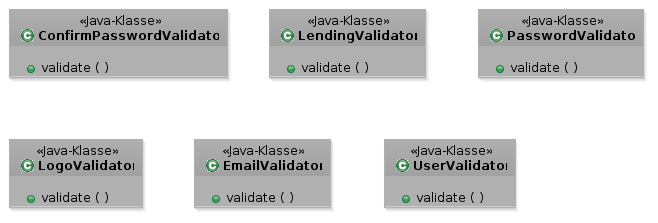
\includegraphics[scale=0.6]{klassendiagramValidator.png}
        \caption{Klassendiagramm des Validator}
        \label{fig:KlassendiagramValidator}
    \end{figure}
%    \end{landscape}


%   \begin{landscape}
    \begin{figure}
        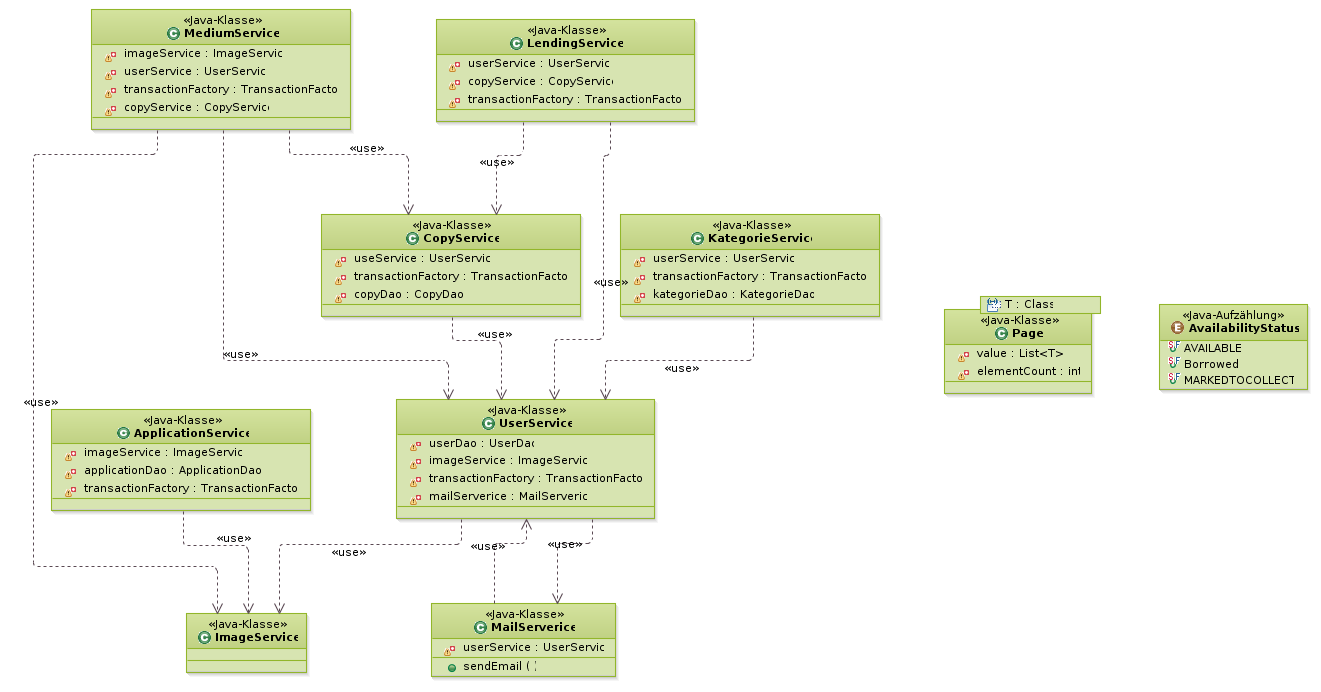
\includegraphics[scale=0.6]{KlassendiagramService.png}
        \caption{Klassendiagramm der Services}
        \label{fig:KlassendiagramService}
    \end{figure}
%    \end{landscape}



 \begin{center}
    \begin{table}
        \begin{tabular} { |p{3,5cm}|p{7,5cm}| }
            \hline
            Java-Klasse & Beschreibung  \\
            \hline\hline
            Medium & Backing Bean für das Erstellen und Bearbeiten eines Medium. \\
            \hline
            AdminConfig & Backing Bean für die Einstellung der Webseite. \\
            \hline
            ChangePassword & Backing Bean für die Änderung des Passwortes. \\
            \hline
            Error & Backing Bean der Seite die Fehlermeldungen anzeigt.\\
            \hline
            Profile & Backing Bean für das Anzeigen und Bearbeiten des Profils eines Benutzers. \\
            \hline
            ForgotPassword & Backing Bean für die Seite, auf der man sich einen neues Passwort zusenden lassen kann, wenn man das altes Passwort vergessen hat. \\
             \hline
            Login & Backing Bean des Logins. \\
             \hline
            Register & Backing Bean für das Anlegen eines neuen Benutzers. \\
            \hline
            Icon & Backing Bean für das Hochladen und Bearbeiten eines Mediums und Logo des Systems. \\
            \hline
            Category & Backing Bean für die Kategorie, die als Liste angezeigt wird. \\
            \hline
            UserList & Backing Bean für die Seite der Benutzersuche. \\
            \hline
            CollectableCopies & Backing Bean der Seite, auf der alle Exemplare abzuholend makiert. \\
            \hline
            DirectLendin & Backing Bean für die Seite der Directausleihe. \\
             \hline
            EmailConfirm & Backing Bean für die Seite der Emailbestätigung. \\
             \hline
            LendingPeriod & Backing Bean für die Seite der Ausleihefrist. \\
             \hline
            MediumSearch & Backing Bean für die Seite der Mediumsuche. \\
             \hline
            ReturnForm & Backing Bean für die Seite der Rückgabe. \\
             \hline
            MediumEdit & Backing Bean für die Seite des Mediumedieren. \\
             \hline
            PrivacyPolicy & Backing Bean für die Seite der Datenschutzerklärung. \\
            \hline
        \end{tabular}
        \end{table}
        \end{center}


\begin{center}
    \begin{table}
        \begin{tabular} { |p{3,5cm}|p{7,5cm}| }
            \hline
            Java-Klasse & Beschreibung  \\
             \hline\hline
            UserDto & Enthält alle Daten des Profils eines Benutzers. \\
            ApplicationDto & Enthält die Daten der Anwendung. \\
            \hline
            MediumDto & Enthält die Daten eines Mediums. \\
            \hline
            CopyDto & Enthält die   Daten eines Exemplar. \\
            \hline
            CategoryDto & Enthält die Daten einer Kategorie. \\
            \hline
            LinkGeneratorDto & Enthält die Daten des Linkgenerators. \\
            \hline
        \end{tabular}
        \end{table}
        \end{center}


  \begin{center}
    \begin{table}
        \begin{tabular} { |p{3,5cm}|p{7,5cm}| }
             \hline
            Java-Klasse & Beschreibung \\
            \hline\hline
            MediumDao & Kontrolliert den Zugriff auf Mediumdaten in der Datenbank. \\
             \hline
            ApplicationDao & Kontrolliert den Zugriff auf die Einstellungen der Anwendung, die in der Datenbank gespeichert sind. \\
            \hline
            UserDao & Kontrolliert den Zugriff auf Benutzerdaten in der Datenbank. \\
            \hline
            CategoryDao & Kontrolliert den Zugriff auf Kategoriedaten in der Datenbank. \\
            \hline
            CopyDao & Kontrolliert den Zugriff auf die Exemplardaten in der Datenbank. \\
            \hline
        \end{tabular}
        \end{table}
        \end{center}


  \begin{center}
    \begin{table}
        \begin{tabular} { |p{3,5cm}|p{7,5cm}| }
             \hline
            Java-Klasse & Beschreibung  \\
           \hline\hline
            EmailValidator & Prüft ob es sich eine gültige E-Mail-Adresse handelt. \\
            \hline
            PasswordValidator & Prüft beim Anlegen eines neuen Benutzerkontos oder beim Ändern des Passwortes, ob das Passwort den Mindestanforderungen entspricht. \\
             \hline
            ConfirmPasswordValidator & Prüft ob die Passwortbestätigung und Passwort übereinstimmen. \\
            \hline
           LogoValidator & Validiert ob eine Datei einem gängigen Bildformat entspricht und nicht zu groß oder auch zu klein ist. \\
             \hline
            UserValidator & Prüft ob eine Ausleihe deren Frist abgelaufen ist. \\
            \hline
            LendingValidator & Prüft ob eine Ausleihe deren Frist abgelaufen ist. \\
            \hline
        \end{tabular}
        \end{table}
        \end{center}


  \begin{center}
    \begin{table}
        \begin{tabular} { |p{3,5cm}|p{7,5cm}| }
              \hline
            Java-Klasse & Beschreibung  \\
           \hline\hline
            ConnectionPool & Verwaltet die Verbindungen zur Datenbank. \\
            \hline
            DatabaseSetup& Erstellt das Datenbankschema und die Verbindung mit Datenbank. \\
             \hline
            SqlTransaction& Wird verwendet, um eine Sql-Transaction zu verarbeiten. \\
             \hline
            DataAcesesException& Wird geworfen,  wenn es keine Verbindung mit Datenbank gibt. \\
           \hline
        \end{tabular}
        \end{table}
        \end{center}


     \begin{center}
       \begin{table}
        \begin{tabular} { |p{3,5cm}|p{7,5cm}| }
             \hline
            Java-Klasse & Beschreibung \\
            \hline\hline
            MediumService &  Service für Aktionen zu Medien. \\
             \hline
            ApplicationService & Service für Aktionen zu der Anwendung. \\
            \hline
            UserService & Service für Aktionen zu dem Benutzer des System. \\
            \hline
            CategoryService & Service für Aktionen zu Kategorie. \\
            \hline
            CopyService& Service für Aktionen zu Exemplaren.\\
             \hline
           LendingService & Service für Aktionen zu der Ausleihe. \\
           \hline
        \end{tabular}
        \end{table}
        \end{center}

\subsection{Paketdiagramm}

    \begin{figure}[h!]
        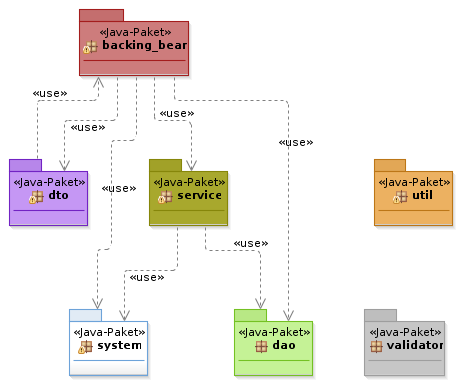
\includegraphics[scale=0.6]{Paketdigram.png}
        \caption{Paketdiagramm}
        \label{fig:Paketdiagramm}
    \end{figure}




%--JSF-Dialoge-----------------------------------------------------------------------------------------------------------------------------------------------------------------------
\section{JSF-Facelets}
\sectionauthor{León Liehr}

% TASK add javadocs
% TASK update AJAX note
% TASK mention query strings and GET/POST parameters!!

\newcommand{\PUB}{jeder}
\newcommand{\ANO}{abgem. Nutzer}
\newcommand{\USR}{angem. Nutzer}
\newcommand{\BIB}{Mitarbeiter}
\newcommand{\ADM}{Administrator}

\newcommand{\component}[2]{\subsubsection{#1 (\texttt{#2})}}
%\newcommand{\page}[2]{\subsubsection{#1, \texttt{#2.xhtml}}}
\newcommand{\page}[2]{
    \subsubsection{#1}
    \paragraph*{Dateipfad} \texttt{#2.xhtml}
}

\newcommand{\Javadoc}{\paragraph*{Javadoc}}

\newcommand{\BTN}{Knopf}
\newcommand{\LNK}{Hyperlink}
\newcommand{\INP}{Eingabefeld}
\newcommand{\PAS}{Passworteingabefeld}
\newcommand{\DRP}{Drop-Down-Liste}
\newcommand{\CHK}{Checkbox}
\newcommand{\OUT}{Ausgabefeld}
\newcommand{\LST}{Paginierte Liste}

\newenvironment{controls}
{
    \begin{table}[H]
        \centering
        \begin{tabular}{ p{7em} p{25em} p{7em} }
            \toprule
            \textbf{Typ} & \textbf{Beschreibung} & \textbf{Sichtbarkeit}\\
            \midrule
        }
        {
            \bottomrule
        \end{tabular}
    \end{table}
}

Sofern nicht anders ausgewiesen folgt jedem Eingabefeld und \PAS ein Ausgabefeld für Meldungen (genauer gesagt eine JSF-\texttt{HtmlMessage}-Komponente), insb. für von JSF-Validatoren geworfene Fehlermeldungen.

% Frage: sind diese Eingabefelder für E-Mails benutzerdef. Komponenten?
% Aufgabe schau dir das Kap zu AJAX im Buch an!!
Aufbauend auf der Voraussetzung einer modernen JavaScript-Implementierung in dem Webbrowser des Clients (Pflichtenheft, Abschnitt 4.1) wird bei Eingabefeldern für E-Mail-Adressen (MANCHER), Signaturen (MANCHER) und Standorten (MANCHER) statt der überholten AJAX-Technologie\footnote{\url{https://xhr.spec.whatwg.org/}} die sog. Fetch API\footnote{\url{https://fetch.spec.whatwg.org/}} verwendet, um während der Eingabe Vorschläge von existierenden Einträgen einblenden zu können.

Mit dem Elementtyp Eingabe wird im Folgenden JSFs \texttt{ui:insert} gemeint.

Zudem werden nachfolgend diese Abkürzungen und Kurzformen verwenden:

% TASK inline table
\begin{table}[H]
\centering
\begin{tabulary}{\textwidth}{RL}
\toprule
%\PUB & jeder \\
\ANO  & abgemeldeter Nutzer \\
\USR & angemeldeter Nutzer \\
\BIB & Bibliotheksmitarbeiter \\
%\ADM & Administrator \\
\bottomrule
\end{tabulary}
\end{table}

\subsection{Komponenten}

%\subsection{Seitenvorlage}

\component{\LST}{PaginatedList}

% TASK attributes, values

\begin{controls}
    \BTN & zum Blättern auf die nächste Seite & \USR\\
    \BTN & zum Blättern auf die vorige Seite & \USR\\
    ?? & ?? values & ??\\
\end{controls}

\component{Editierbarer Text}{EditableText}

Das Attribut der Komponente ist der Text.

% QUESTION visibility as an attribute, too?? if yes, how???

\begin{controls}
    \OUT & für das Textattribut & \PUB\\
    \INP & für das Textattribut & \ADM\\
\end{controls}

\subsection{Seitenvorlagen (Templates)}

\page{Einzige Seitenvorlage}{public/template}\label{template}

\begin{controls}
    Einlage & des Titels einer konkreten Seite & \PUB\\
    Einlage & des Inhalts einer konkreten Seite & \PUB\\
    \BTN & zum Anzeigen der kontextsensitiven Hilfe; als Fragezeichenbildsymbol dargestellt & \PUB\\
    \LNK & zu der erweiterten Suche & \PUB\\
    \INP & für die Mediensuche; alleinig die Betätigung der Eingabetaste sendet ab & \PUB\\
    \LNK & zu der Profilseite & \USR\\
    \LNK & zum Abmelden; zur Anmeldemaske & \USR\\
    \LNK & zur Anmeldemaske & \ANO\\
    \LNK & zur Registrierungsseite  & \ANO\\
    \LNK & zu den abzuholenden Exemplaren & \BIB\\
    \LNK & zu der Medienrückgabe & \BIB\\
    \LNK & zu der Direktausleihe & \BIB\\
    \LNK & zu der Verwaltung & \ADM\\
    \OUT & für globale Meldungen (JSFs \texttt{HtmlMessages}) & \PUB\\
    \LNK & zur Datenschutzerklärung & \PUB\\
    \LNK & zum Impressum & \PUB\\
    \LNK & zum Kontakt & \PUB\\
\end{controls}

\subsection{Seiten}

Alle Seiten nehmen die einzige Seitenvorlage (\ref{template}) als Vorlage.
Jede Seite wird vom einer entsprechenden Backing Bean angetrieben, welche sich namentlich lediglich durch die Schreibweise unterscheidet. So wird bspw. die Seite \texttt{privacy-policy.xhtml} (in \textit{dash case}) mit der Bean \texttt{PrivacyPolicy} (in \textit{upper camel case}) assoziiert.

\page{Abzuholende Exemplare}{staff/copies-ready-for-pickup}

\Javadoc
This page is used by library staff to be up to speed regarding which copies are ready to be picked up and
whether they can expect someone to soon enter the library and arrive at their counter.

\begin{controls}
    \LST & aller abzuholenden Exemplare & \BIB\\
\end{controls}

\page{Eigene abzuholende Exemplare}{account/my-copies-ready-for-pickup}

\Javadoc
On this page a user gets to know which copies they want to pick up from the library and borrow thereafter
and how much time they have left to do so until they exceed the deadline.

\begin{controls}
    \LST & aller abzuholenden Exemplare & \USR\\
\end{controls}

\page{Eigene ausgeliehene Exemplare}{account/my-borrowed-copies}

\Javadoc
This page informs the user which copies they borrowed from the library and how much time they still have left
until they have to return them to not exceed the deadline.

\begin{controls}
    \LST & aller ausgeliehenen Exemplare & \USR\\
\end{controls}

\page{Anmeldemaske}{public/login}

\Javadoc
This page is the one users first face when they are not already logged in.
It allows them to log into the system to gain the privilege to borrow copies.
If a logged-in user accesses this page by manually entering its URL, a message is shown instead of the
login form and they get automatically redirected to their profile page.

\begin{controls}
    \INP & für die E-Mail-Adresse & \ANO\\
    \PAS & & \ANO\\
    \BTN & zum Anmelden & \ANO\\
    \BTN & zum Passwortzurücksetzen; als \LNK dargestellt, um unauffälliger zu sein, da es eine zweitrangige Aktion ist & \ANO\\
\end{controls}

\page{Datenschutzerklärung}{public/privacy-policy}

\Javadoc
This page declares the privacy policy of this system.

\begin{controls}
    \OUT & für die Datenschutzerklärung & Nicht-\ADM\\
    \INP & für die Datenschutzerklärung & \ADM\\
    \BTN & zum Speichern der Änderungen & \ADM\\
\end{controls}

\page{Direktausleihe}{staff/direct-lending}

\Javadoc
This page enables staff to lend a person most probably in front of their counter a series of copies.
It is intended but not a hard requirement that library staff scans the copies given to them by the customer with a dedicated device which automatically pastes the signatures into the relevant input fields. Analogously with the email address stored inside of their membership card.

\begin{controls}
    \INP & für die E-Mail-Adresse des Ausleihenden & \BIB\\
    \INP & für die Signatur eines auszuleihenden Exemplars; beim Laden der Seite fünfmal vorhanden. Durch das Pressen des relevanten Knopfs wird ein weiteres Feld angehängt & \BIB\\
    \BTN & zum Hinzufügen eines weiteren Signaturfelds & \BIB\\
    \BTN & zum Ausleihen & \BIB\\
\end{controls}

\page{E-Mail-Bestätigung}{public/email-confirmation}

% BEACON TASK BEACON docs etc

% TASK PARAM TOKEN

\Javadoc
Accessing this page potentially verifies the email address of a specific user. For this,
it takes a verification token as a query parameter. If absent or invalid, nothing user-facing happens.
This secures against certain attacks.

%\begin{controls}
%    \BTN & zur Bestätigung der E-Mail-Adresse & \PUB\\
%\end{controls}

\page{Fehlerseite}{public/error}

\Javadoc
The sink for all kinds of fatal errors that happened in the system.
They are either caused client-side (HTTP status codes 4XX) or server-side (HTTP status codes 5XX).
If it's a client-side error, the user gets redirected to either the login page or their profile depending on if they are logged in or not. The redirection happens after some fixed amount of time.

\begin{controls}
    \OUT & für den Titel der Fehlermeldung & \PUB\\
    \OUT & für die Beschreibung des Fehlers & \PUB\\
\end{controls}

\page{Impressum}{public/site-notice}

\Javadoc
This page contains the site notice.

\begin{controls}
    \OUT & für das Impressum & Nicht-\ADM\\
    \INP & für das Impressum & \ADM\\
    \BTN & zum Speichern der Änderungen am Impressum & \ADM\\
\end{controls}

\page{Kategorienbearbeitung}{staff/category-editor}

% Task: rephrase
\Javadoc The category editor allows the creation and modification of a category.
Only library staff and administrators are allowed to access this page.
This page should only be accessed from the category browser, otherwise the required parameters
are likely missing which would be an error.
This page can be reached when library staff clicks on the edit button next to a category's name in the browser.
In this case, the identifier of the category to be edited is transmitted as a parameter.
This page can be reached when library staff clicks on the create button in the context of a category.
In that case, the identifier of the category to be treated as the parent of the new category is transmitted
as a parameter.

\begin{controls}
    \INP & für den Kategorienamen & \BIB\\
    \INP & für die Kategoriebeschreibung & \BIB\\
    \BTN & zum Speichern der Änderungen & \BIB\\
\end{controls}

\page{Kategorierenstöberer}{public/category-browser}

\Javadoc
This page offers users to browse through all available categories mediums are part of in a structured manner.
It renders it possible for the consumer to discover new mediums.

\begin{controls}
    \INP & für den Suchterm der Kategoriensuche & \PUB\\
    \BTN & zum Durchführung der Suche & \PUB\\
    \LNK & zur Kategorienbearbeitung (Erstellung einer neuen) & \BIB\\
    \LNK & zur Kategorienbearbeitung & \BIB\\
    \BTN & zum Löschen der Kategorie; zur Elterkategorie & \BIB\\
    \LNK & zur Medienerstellung unter der aktuellen Kategorie & \BIB\\
\end{controls}

\page{Kontakt}{public/contact}

\Javadoc The contact form allows any user to get in touch with the library staff.
Anonymous users have to enter their email address for staff to be able to reply.
If the user is logged in, the information is simply taken from their account data.

\begin{controls}
    Textbereich & für die Frage & \PUB\\
    \INP & für die E-Mail-Adresse & \ANO\\
    \INP & für den vollständigen Namen & \ANO\\
    \INP & für den Ort/die PLZ & \ANO\\
    \BTN & zum Absenden & \PUB\\
\end{controls}

\page{Leihfristverstöße}{admin/lending-period-violations}

\begin{controls}
    \LST & von Exemplaren und Nutzern & \ADM\\
\end{controls}

\page{Medienerstellung}{staff/medium-creation}

\begin{controls}
    \INP & für ein Medienattribut; existiert pro Medienattribut & \BIB\\
    Zeitdauereingabefeld & für die Rückgabefrist & \BIB\\
    \INP & für den Standort eines neuen Exemplars & \BIB\\
    \INP & für die Signatur eines neuen Exemplars & \BIB\\
    \BTN & zum Anlegen des neuen Mediums und des ersten Exemplars & \BIB\\
\end{controls}

\page{Medienrückgabe}{staff/return}

\begin{controls}
    \INP & für die E-Mail-Adresse des Abgebenden & \BIB\\
    \INP & für die Signatur eines abzugebenden Exemplars; beim Laden der Seite fünfmal vorhanden. Durch das Pressen des relevanten Knopfs wird ein weiteres Feld angehängt & \BIB\\
    \BTN & zum Hinzufügen eines weiteren Signaturfelds & \BIB\\
    \BTN & zum Abgeben & \BIB\\
\end{controls}

\page{Mediensuche}{public/media-search}

\begin{controls}
    \INP & für den Suchterm der freien Suche & \PUB\\
    \BTN & zur Durchführung der Suche & \PUB\\
    \DRP & für den Suchoperator; beim Laden der Seite dreimal vorhanden (je gruppiert mit Suchkriterium und -feld) & \PUB\\
    \DRP & für das Suchkriterium; beim Laden der Seite dreimal vorhanden (je gruppiert mit Suchoperator und -feld) & \PUB\\
    \INP & für den Suchterm der differenzierten Suche; beim Laden der Seite dreimal vorhanden (je gruppiert mit Suchoperator und -kriterium) & \PUB\\
    \BTN & zum Hinzufügen eines weiteren Gruppe aus Suchoperator, -kriterium und -feld & \PUB\\
    \LST & aller Suchergebnisse (falls vorhanden) & \PUB\\
\end{controls}

\page{Mediumsansicht}{public/medium}

% TASK DONT USE A PAGINATED LIST HERE!!! UPDATE THE STUFF!!!

\begin{controls}
    \LNK & zurück zur Trefferliste / Mediensuche; nur sichtbar, falls der Nutzer von der Suche kommt & \PUB\\
    % TASK und Nicht-Admin
    \OUT & für ein Medienattribut; existiert pro Medienattribut & Nicht-\BIB\\
    \INP & für ein Medienattribut; existiert pro Medienattribut & \BIB\\
    \BTN & zum Speichern der Änderungen an den Medienattributen & \BIB\\
    \BTN & zur Bindung an die Abholung des Mediums; nur sichtbar, falls es dem Nutzer erlaubt ist auszuleihen & \USR\\
    \OUT & für die Rückgabefrist; bezieht auch die nutzerbezogene Frist ein, anders als das \INP{} darunter & \USR\\
    \INP & für die Rückgabefrist & \BIB\\
    \BTN & zum Speichern der Änderungen an der Rückgabefrist & \BIB\\
    \LNK & zum Löschen des Mediums; zur zuvor aufgerufenen Seite & \BIB\\
    \LST & aller Exemplare & \PUB\\
    \OUT & für den Standort eines Exemplars; existiert pro Exemplar & \PUB\\
    \INP & für den Standort eines Exemplars; existiert pro Exemplar & \BIB\\
    \OUT & für die Signatur eines Exemplars; existiert pro Exemplar & \PUB\\
    \INP & für die Signatur eines Exemplars; existiert pro Exemplar & \BIB\\
    \BTN & zum Speichern der Änderung am Exempla; existiert pro Exemplar & \BIB\\
    \BTN & zum Löschen eines Exemplars; existiert pro Exemplar in der Tabelle & \BIB\\
    \BTN & zum Stornieren einer Abholung; existiert pro Exemplar in der Tabelle & \BIB\\
    \LNK & zur Direktausleihe; existiert pro Exemplar in der Tabelle & \BIB\\
    \BTN & zur Bindung an die Abholung des Mediums; existiert pro Exemplar in der Tabelle; nur sichtbar, falls es dem Nutzer erlaubt ist auszuleihen & \USR\\
    \INP & für den Standort eines neuen Exemplars & \BIB\\
    \INP & für die Signatur eines neuen Exemplars & \BIB\\
    \BTN & zum Erstellen eines Exemplars & \BIB\\
\end{controls}

\page{Mediumschemabearbeitung}{admin/medium-schema-editor}

\begin{controls}
    \INP & für den Namen eines Attributs; existiert pro Attribut & \ADM\\
    \DRP & für den Typen eines Attributs; existiert pro Attribut & \ADM\\
    \DRP & für die Position in der Medienvorschau; existiert pro Attribut & \ADM\\
    \BTN & zum Löschen eines Attributes; existiert pro Attribut & \ADM\\
    \BTN & zum Hinzufügen eines weiteren Gruppe aus \INP{}ern und \DRP{}n & \ADM\\
    \BTN & zum Speichern der Änderungen & \ADM\\
\end{controls}

\page{Nutzersuche}{admin/user-search}

\Javadoc
This page enables administrators to search for users.

\begin{controls}
    \INP & für den Suchterm & \ADM\\
    \BTN & zur Durchführung der Suche & \ADM\\
    \CHK & für das Einschränken auf gesperrte Nutzer & \ADM\\
    \LST & aller Suchergebnisse (falls vorhanden) & \ADM\\
\end{controls}

\page{Passwortzurücksetzung}{public/password-reset}

%TASK rephrase
\Javadoc
This page is reached by a user when they click on the link they received in an email.
For the mechanisms to work, it takes a token as a query parameter.
After submitting the form, the user is not logged into the system yet, they are redirected to the login form.
This secures against certain attacks.
If the token is absent or invalid, nothing user-facing is going to happen: Clicking the button still means redirection to the login page.

\begin{controls}
    \PAS & für das neue Passwort & \PUB\\
    \PAS & zur Bestätigung des neuen Passworts & \PUB\\
    \BTN & zum Zurücksetzen des Passworts; zur Anmeldemaske & \PUB\\
\end{controls}

\page{Profilseite}{account/profile}

% expand
\Javadoc
This page is either the profile page of the current user or if it is an administrator possibly also
of a user different from the logged-in one.
It allows a user to change their personal information the system stores and it allows administrators to manage other accounts.

\begin{controls}
    % BEACON TASK BEACON \INP_OR_OUT (new component)
    \INP & für den Vornamen & \USR\\
    \INP & für den Nachnamen & \USR\\
    \PAS & für das Passwort & \USR\\
    \PAS & zur Bestätigung & \USR\\
    \INP & für die E-Mail-Adresse & \USR\\
    \INP & für den Ort & \USR\\
    \INP & für die PLZ & \USR\\
    \INP & für die Straße& \USR\\
    \INP & für die Hausnummer & \USR\\
    \DRP & für die Nutzerrolle & \ADM\\
    \CHK & zum Sperren des Nutzers & \ADM\\
    \INP & für die Rückgabefrist & \ADM\\
    \BTN & zum Speichern der Änderungen an den Benutzerdaten & \USR\\
    \LNK & zu den abzuholenden und ausgeliehenen Exemplaren & \USR\\
    \BTN & zum Schließen des Accounts; zur Anmeldemaske & \USR\\
    \BTN & zum Löschen des Nutzers; zur Verwaltungsseite & \ADM\\
\end{controls}

\page{Registrierungsseite}{public/registration}

\begin{controls}
    \INP & für den Vornamen & \USR\\
    \INP & für den Nachnamen & \USR\\
    \PAS & & \USR\\
    \PAS & zur Bestätigung & \USR\\
    \INP & für die E-Mail-Adresse & \USR\\
    \INP & für den Ort & \USR\\
    \INP & für die PLZ & \USR\\
    \INP & für die Straße & \USR\\
    \INP & für die Hausnummer & \USR\\
    \DRP & für die Nutzerrolle & \ADM\\
    \BTN & zum Registrieren des Accounts & \ANO/\ADM\\
\end{controls}

\page{Verwaltungsseite}{admin/administration}

\begin{controls}
    \INP & für die Rückgabefrist & \ADM\\
    \INP & für den Mahnungszeitpunkt & \ADM\\
    \INP & für die Abholfrist & \ADM\\
    \INP & für den Systemnamen & \ADM\\
    \CHK & für den Zugangsstatus (anonym oder nicht) & \ADM\\
    \CHK & für den Registrierungsstatus & \ADM\\
    \INP & für den regulären Ausdruck valider E-Mail-Adressen & \ADM\\
    \DRP & für das Farbschema des Systems & \ADM\\
    Datei-Upload & für das Logo des Systems & \ADM\\
    \BTN & zum Speichern der Änderungen an den Systemeinstellungen & \ADM\\
    \LNK & zu der Medienerstellung & \ADM\\
    \LNK & zu der Registrierungsseite (fremden Nutzer erstellen) & \ADM\\
    \LNK & zur Mediumsschemabearbeitung & \ADM\\
    \LNK & zu den Leihfristverstößen & \ADM\\
    \LNK & zu der Nutzersuche & \ADM\\
    \INP & für den Suchterm einer Nutzersuche & \ADM\\
    \BTN & zum Durchführung der Suche & \ADM\\
\end{controls}

%--Systemfunktionen----------------------------------------------------------------------------------------------------------------------------------------------------------------
\section{Systemfunktionen}
\sectionauthor{Jonas Picker}
\subsection{Technische Systemsicherheit}
\noindent \textbf{Kommunikationserschlüsselung:} Durch die CA-Zertifizierung des Servers wird eine TLS-Trans-portverschlüsselung bei der Kommunikation zwischen Klient und Server verwendet. Ist die Datenbank, wie im Pflichtenheft (Abschnitt 4.3  'Server') beschrieben, über SSL-VPN angebunden, ist die Kommunikation zwischen ihr und dem Server ebenfalls verschlüsselt. \\
\textbf{Nutzerberechtigungen:} Für die Überprüfung der Zugangsberechtigungen bei jeder HTTPS-Anfrage implementiert die Klasse !!!\hyperlink{}{}!!! das PhaseListener-Interface, welches zu implementierende Methoden zum Ausführen von Code vor oder nach jeder Phase des JSF-Life-Cycle vorgibt. In unserem Fall wird am frühestmöglichen Punkt (vor der Restore-View-Phase) geprüft, ob der Anfragesteller auch berechtigt ist, die vorhergesehene Antwort vom Server zu erhalten. Aus Redundanzgründen verwenden wir für Seiten, auf die mehrere Nutzerrollen Zugriff haben, die gleichen Facelets. In den jeweiligen Backing-Beans wird dann, durch Zugriff auf die von JSF getrackte Nutzer-Session der Klasse  !!!\hyperlink{}{}!!!, die Rolle des Benutzers überprüft. Für jeden Seitenbesucher werden dann nur die rollenspezifischen Knöpfe und Anzeigen gerendert (siehe !!!\hyperlink{}{auch}!!!). Durch die inklusive Rollenhierarchie lassen sich so alle Funktionalitäten der Rollen im gleichen Facelet einbinden.\\
\textbf{Session-Hijacking\footnote{Das Stehlen einer validen Nutzer-Session um Zugriff auf den Account und seine Berechtigungen zu erhalten}:} Um diesen Angriffsvektor zu schützen, wird der Identifikator der Nutzer-Session an kritischen Stellen (z.B. nach dem Login) manuell ausgetauscht. \\
\textbf{Cross-Site-Scripting\footnote{Auch XSS: das Einschleusen von browserinterpretierbarem HTML-Code auf ungesicherte Teile einer Website}:} Das Escapen von HTML-Sonderzeichen wird von JSF bei allen nutzergenerierten Teilen der Anwendung unterstützt. Alle Elemente der JSF-Facelets, die nutzergenerierten In- und Output weitergeben, haben den impliziten Standartwert 'escape=true'. Da wir diesen in unserer Implementierung nie manuell auf 'false' setzen, ist XSS in dieser Applikation unmöglich. \\
\textbf{SQL-Injection\footnote{Einschleusen von SQL-Code in Formularfelder, um Zugriff auf die Datenbank zu erhalten}:} Durch das Konsequente Verwenden der 'Prepared Statements' in unserer !!!\hyperlink{}{Datenzugriffsschicht}!!! beugen wir SQL-Injections vor. Diese JDBC-Funktionalität trennt das eigentliche SQL-Statement von den nutzergenerierten Parametern und Verhindern so das Ausführen von maliziösem SQL-Code in der Datenbank. \\
\subsection{Logging}
Mit der Klasse !!!\hyperlink{}{}!!! ist unser System mit einer eigenen Log-Funktion ausgestattet. Diese dient sowohl zum Debugging während der Entwicklung, als auch zum Protokollieren der Fehler und Abläufe im laufenden System. Durch Setzten der Variable 'LOG\_CONSOLE: ' mit den Werten 'TRUE' oder 'FALSE' kann eingestellt in der Konfigurationsdatei werden, ob die Meldungen auch in Echtzeit auf der Konsole ausgegeben oder nur in das Log-File geschrieben werden. Es gibt drei Log-Level, zwischen denen, durch Setzen der Variable 'LOG\_LEVEL: ' mit einem der unten aufgeführten Werte, beim Systemstart umgeschaltet werden kann. Die folgenden Kategorien sind inklusiv, die Letzte schließt somit die oberen beiden mit ein. \\
\textit{'SEVERE':} Diese Einstellung des Loggers protokolliert nur schwere Fehler, die unmittelbare Konsequenzen für den Anwendungsbetrieb haben. Um ein schnelles Volllaufen des Log-Files zu vermeiden, ist dies die Standarteinstellung.\\
\textit{'DETAILED':} Fehler und fehlgeschlagene Prozeduren, die die Integrität der Anwendung nicht gefährden, werden zusätzlich protokolliert.\\
\textit{'DEVELOPMENT':} Hierunter fallen sowohl Protokollierungen von erfolgreichen oder seltenen Abläufen, alsauch sonstige nützliche Meldungen. Da das Log-File schnell sehr groß und unübersichtlich werden könnte, empfehlen wir, diese Option nur bei Problemen zu wählen.\\
\subsection{Selbstständige Abläufe}
Die Klasse !!!\hyperlink{}{}!!! ermöglicht dem System, selbstständig in einstellbaren Abständen Wartungsaufgaben durchzuführen. Alle unten aufgelisteten Aufgaben sind somit von der der aktuellen Systemzeit des Servers abhängig und werden darüberhinaus nur mit einer maximalen zeitlichen Unsicherheit des gewählten Intervalls durchgeführt. Die Einstellung wird beim Systemstart durch den gesetzten Wert der Variable 'SCAN\_INTERVAL: ' bestimmt. Der von uns empfohlene Standartwert repräsentiert eine Minute, sollten Sie diesen verlängern wollen tragen Sie stattdessen eine andere positive ganze Zahl ein. Der Wartungsthread vergleicht die Operationsfrist der zur Abholung markierten Exemplare mit der aktuellen Systemzeit und setzt bei Überschreitung den Verfügbarkeitsstatus wieder auf 'verfügbar'. Bei Exemplaren mit dem Status 'ausgeliehen' wird, zusätzlich zur Frist, die Mahnungsversatzzeit beachtet und bei Bedarf die Klasse !!!\hyperlink{}{}!!! zum Versenden einer E-Mail angestoßen. Die abgelaufenen Tokens der Benutzer-Tabelle werden ebenfalls gelöscht.
\subsection{Datenbankverbindung}
Wenn die Java Laufzeitumgebung des Systems plötzlich beendet wird und das System abstürzt, wird trotzdem mittels einer ShutdownHook noch das Schließen offener Datenbankverbindungen versucht. Außerdem wird durch das logische Zusammenfassen der voneinander abhängigen Datenbanktransaktionen in den Steuermethoden der !!!\hyperlink{}{DAOs}!!! sichergestellt, dass das ACID-Prinzip bestmöglich eingehalten und die Datenbank im Fehlerfall in einem konsistenten Zustand hinterlassen wird. Dies ist jedoch (z.B. bei einem Stromausfall) nicht immer möglich.
\subsection{Starten und Stoppen der Anwendung}
\noindent \textbf{Start:} Durch Implementierung des SystemEventListener-Interface werden beim Systemstart von der Klasse!!!\hyperlink{}{}!!! alle weiteren Aktionen angestoßen. Die Initialisierung des !!!\hyperlink{}{Loggers}!!! geschieht zuerst, danach wird die Konfigurationsdatei eingelesen, das Log-Level und der gewählte Konsolenausgabemodus gesetzt und mit den restlichen Parametern eine !!!\hyperlink{}{eigene Initialisierungsklasse}!!! für Prozesse der !!!\hyperlink{}{Datenzugriffsschicht}!!! aufgerufen, in der zunächst die Datenbankverbindung überprüft wird. Sollten die Verbindung fehlschlagen, wird, ähnlich zu !!!\hyperlink{}{diesem Prozess}!!!, eine Fehlermeldung ausgegeben/geloggt. Im Erfolgsfall wird dann überprüft, ob die benötigten Tabellenstrukturen bereits vorhanden sind. Falls nicht wird das manuelle Anlegen der Tabellen (Mediumsschema wird mit dem \hyperlink{Standartattributsatz}{Standartattributsatz} befüllt) über einen Konsoleninput mit 'Y' oder 'N' entschieden werden müssen. Bei existierenden Tabellen wird  nun der !!!\hyperlink{}{Connection-Pool}!!! initialisiert und der Startprozess der !!!\hyperlink{}{Datenzugriffsschicht}!!! ist abgeschlossen. Es wird nun das zuvor ausgewählte \hyperlink{Farbschemaattribut}{Farbschema} aus der Datenbank abgefragt, an die !!!\hyperlink{}{darüberliegende Schicht}!!! weitergeleitet und von !!!\hyperlink{}{dort}!!! aus der !!!\hyperlink{}{Wartungsthread}!!! aktiviert und das ausgewählte Farbschema eingestellt, danach ist das System betriebsbereit. \\
\textbf{Stop:} 
Beim planmäßigen Herunterfahren des Systems durch das Ausschalten des Tomcat auf dem Server (z.B. via shutdown.sh) reicht die Klasse !!!\hyperlink{}{}!!! eine Nachricht an die Klasse !!!\hyperlink{}{}!!!, von wo aus zunächst der !!!\hyperlink{}{Wartungsthread}!!! beendet und danach die noch offenen Datenbankverbindungen über den !!!\hyperlink{}{Connection-Pool}!!! geschlossen werden. Nach Durchreichen der Erfolgsmeldung nach oben, wird die Anwendung gestoppt. Nutzersessions überleben das Ausschalten des Servers nicht.

%--Datenfluss--------------------------------------------------------------------------------------------------------------------------------------------------------------------------
\section{Datenfluss}
\sectionauthor{Sergei Pravdin}
Die Kommunikationen zwischen den Klassen und die Interaktionen des Systems werden durch den Sequenzdiagramme abgebildet. Um einen Datenfluss beispielhaft zu zeigen, werden die zwei Szenarien vorgelegt. Zuerst bucht ein angemeldeter Nutzer ein Medium-Exemplar erfolgreich zur Ausleihe. Im zweiten Szenario bucht ein angemeldeter Nutzer ein Medium-Exemplar erfolglos zur Ausleihe, weil die Verbindung mit der Datenbank fehlgeschlagen ist.
\subsection{Interaktionen beim erfolgreichen Buchen eines Medium-Exemplars}
Der Nutzer befindet sich auf der Mediensuche-Seite und wünscht das Buch 'Programmieren lernen' zu buchen. Im System existiert das Medium mit dem Titel 'Programmieren lernen' und der Signatur '17RE'. Ein Exemplar mit der Signatur '17RE (+1)' gehört zu dem genannten Medium. Das System ist so eingestellt, dass die angemeldeten Nutzer Zugriff auf den Medien haben.
\subsubsection{Suchen nach dem Medium}
Der Nutzer gibt 'Programmieren lernen' und '17RE' in die Suchfelder 'Titel' und 'Signatur' und klickt auf den Suchen-Button. Das Mediensuche-Bean kapselt die Sucheingabe ins Mediensuche-DTO ein. Das Mediensuche-DTO ruft die Methode 'getMedien' aus dem Mediensuche-DAO auf. Das Mediensuche-DAO ruft die Methode 'getConnection' aus dem Connection-Pool-Bean und bekommt eine Connection von dem zurück. Danach führt das Mediensuche-DAO eine selectSQL-Anfrage durch und gibt eine Liste der entsprechenden Medien dem Mediensuche-DTO zurück. Im nächsten Schritt leitet Mediensuche-DTO diese Liste der Medien dem Mediensuche-Bean weiter. Das Mediensuche-Bean ruft seine Methode 'updateMedien' auf und gibt dem Nutzer die aktualisierte Mediensuche-Seite zurück.
\subsubsection{Navigation zum Medium}
Der Nutzer klickt auf das angezeigte Medium 'Programmieren lernen'. Das Mediensuche-Bean ruft die Methode 'navigate' auf und gibt die Mediumsansicht-Seite zurück.
\subsubsection{Buchen eines Exemplares}
Der Nutzer klickt auf den Buchen-Button. Das Medium-Bean ruft die Methode checkStatus aus dem UserSession-Bean auf, um zu prüfen, ob der Nutzer Zugriff zum Buchen hat. Das UserSession-Bean gibt das positive Ergebnis dem Medium-Bean zurück. Das Medium-Bean kapselt das Buchen ins Medium-DTO ein und das Medium-DTO ruft die Methode book() aus dem Medium-DAO auf. Das Medium-DAO ruft die Methode 'getConnection' aus dem Connection-Pool-Bean und bekommt eine Connection von dem zurück. Danach führt das Medium-DAO eine updateSQL-Anfrage durch. Im nächsten Schritt gibt Medium-DTO  dem Medium-Bean das Ergebnis der Operation zurück. Das Medium-Bean ruft seine Methode 'updateExamples' auf und gibt dem Nutzer die aktualisierte Medium-Seite zurück. Das Exemplar ist erfolgreich gebucht.

\newpage
\newgeometry{left=0cm,right=0cm,top=0.5cm,bottom=0cm}

\begin{figure}[h]
    \centering
    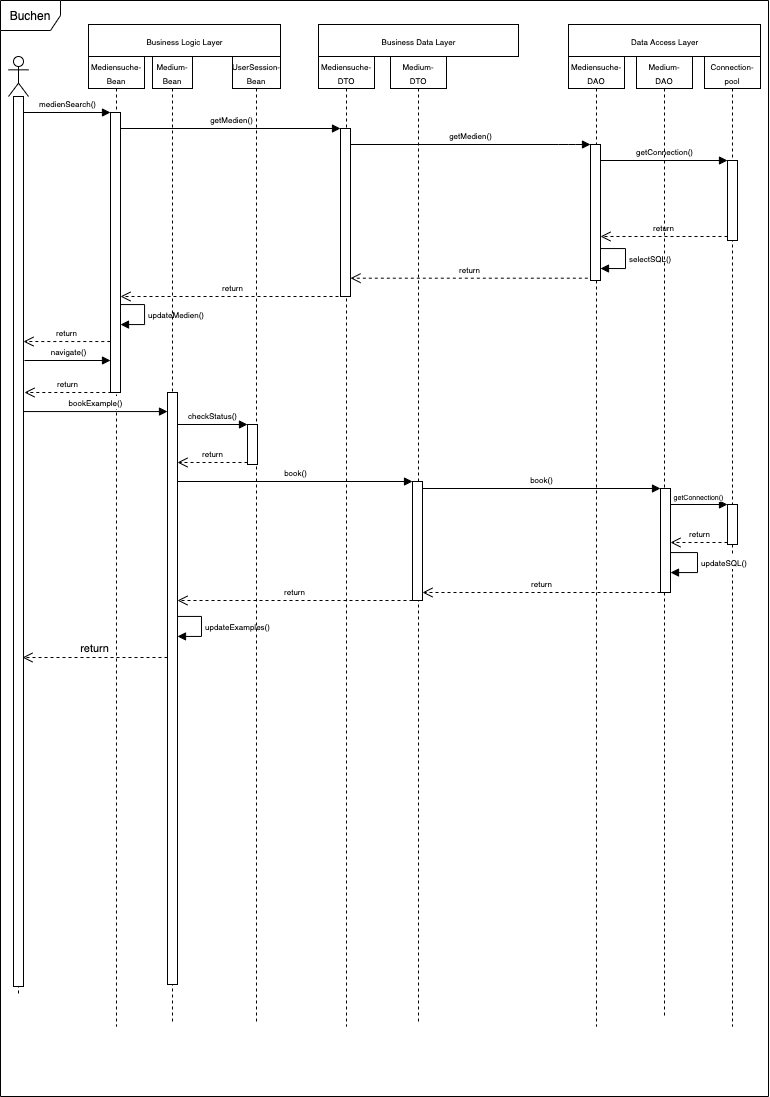
\includegraphics[width = 45em]{Sequenzdiagramm-2}
    \caption{Interaktionen bei einem erfolgreichen Buchen eines Medium-Exemplars}
    \label{Sequenzdiagramm}
\end{figure}

\restoregeometry
\newpage

%--ER-Modell--------------------------------------------------------------------------------------------------------------------------------------------------------------------------
\section{ER-Modell}
\sectionauthor{Jonas Picker}

\newgeometry{left=0cm,right=0cm,top=0cm,bottom=0cm}

\begin{figure}[h]
    \hypertarget{ERDia}{}
    \centering
    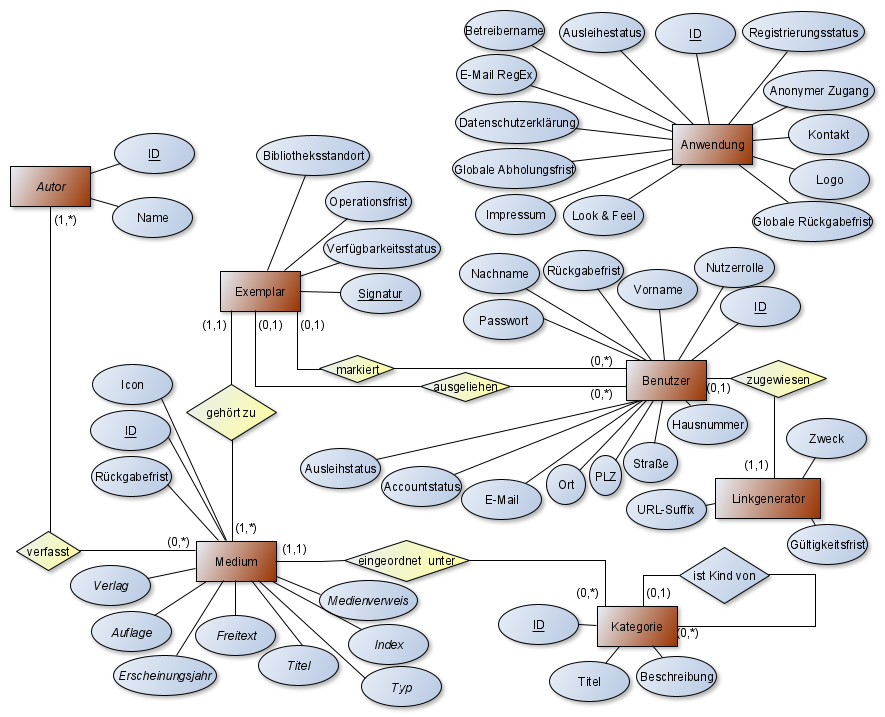
\includegraphics[angle = 270, width = 60em]{ER-Diagramm}
    \caption{Entity-Relationship Diagramm}
    \label{ER-Diagramm}
\end{figure}

\restoregeometry
\newpage

\subsection{Legende}
Beschreibung des \hyperlink{ERDia}{ER-Diagramms}: \\
\\
\textbf{Medium:} Diese Entität modelliert die von der Bibliothek verwalteten Medien. Außer des Primärschlüssels besitzt sie mindestens ein zugehöriges Exemplar und eine variable Anzahl von Attributen. Der \hypertarget{Standartattributsatz}{Standartattributsatz} für Medien wird unten aufgeführt. Es können benutzerdefinierte Attribute hinzugefügt werden (PfHft. /F380/) und jedes der folgenden Attribute ist löschbar (PfHft. /F381/):
\begin{center}
\begin{tabular} { c c c }
Titel & Erscheinungsjahr &  Verlag \\
 Medientyp & Version &  Freitext \\
 Autoren &  Index (ISBN/ISSN) &  Link auf elektronische Version \\
\end{tabular}
\end{center}
\textbf{Attribut:} Diese schwache Entität hält den Namen und Wert eines Medienattributs, ihr ist genau ein Attributtyp zugeordnet.\\
\textbf{Attributtyp:} Vom Attribut abhängige, schwache Entität. Hiermit werden dem Attribut zugehlrige Eigenschaften modelliert. 'Vorschauposition' bestimmt, ob und an welcher Stelle das Attribut in der Medienvorschau (z.B. in der Listenansicht der Suchergebnisse) angezeigt werden soll. 'Multiplizität' entscheidet, ob das zugehörige Attribut mehrfach pro Medium mit unterschiedlichen Werten vorkommen kann oder nicht. 'Persistenz' ist eine Markierung für Attribute, die nicht zum modifizierbaren Attributsatz gehören (z.B. die Rückgabefrist für Medien). 'Datentyp' beschreibt die im Attributwert gespeicherten Daten (z.B. 'String' für Textattribute oder 'Image' um Bilder zu speichern). \\
\textbf{Kategorie:} Die mit dieser Entität verbundenen Relationen ordnen jedem Medium genau eine Kategorie zu und modellieren die Kategoriehierarchie (PfHft. /W440/) durch die Selbstbeziehung. Es wird einen unlöschbaren Top-Knoten in der Hierarchie geben, zu dem alle Medien, die nie in eine Kategorie eingeteilt wurden oder deren Kategorie gelöscht wurde, gehören. Sollten alle Medien in benutzerdefinierten Kategorien stecken, hat der Top-Knoten keine zugeordneten Medien und nimmt somit nicht an der 'eingeordnet unter'-Relation teil.\\
\textbf{Exemplar:} Diese schwache Entität ist vom zugehörigen Medium abhängig. Ein bestimmtes Exemplar kann von genau einem Nutzer zur Abholung markiert oder ausgeliehen werden, diese Aktionen schließen sich gegenseitig aus (PfHft. /F310/) und ändern (genau wie eine Rückgabe) den Verfügbarkeitsstatus und die dazugehörige Operationsfrist dementsprechend. 'Signatur' und 'Bibliotheksstandort' halten bibliothekspezifische Kodierungen. \\
\textbf{Benutzer:} Ob ein Benutzer die Ausleihfunktion benutzen kann, wird durch das Attribut 'Ausleihsperre' modelliert. 'Verifizierungsstatus' zeigt hingegen an, ob der Nutzeraccount bereits den Verifizierungsprozess durchlaufen hat (PfHft. /W70/). Das Passwort wird in gehashter Form abgespeichert. Zur Passwortzurücksetzung und E-Mail-Verifikation wird pro Nutzer ein begrenzt gültiges, einzigartiges 'Token' verwendet, um den entsprechenden Link zu bauen. Die 'Rückgabefrist' für Ausleihen eines Benutzers wird ebenfalls modelliert.\\
\textbf{Registrierter Nutzer:} Diese Nutzer haben positiven 'Verifizierungsstatus'.\\
\textbf{Bibliotheksmitarbeiter:} Diese Entität modelliert die Rolle der Bibliotheksmitarbeiter.\\
\textbf{Administrator:} Diese Entität modelliert die Rolle der Administratoren. Die von der Benutzerentität ausgehende Hierarchie soll die inklusiven Rollen im System modellieren.  \\
\textbf{Adresse:} Vom Benutzer abhängig. Enthält die Bestandteile einer Nutzeradresse als Attribute. \\
\textbf{Anwendung:} Hier werden die setzbaren globalen Variablen und Anwendungseinstellungen modelliert. 'Anonymer Zugang' bestimmt die Berechtigungen anonymer Nutzer beim Besuchen des Webspaces (PfHft. /F10/), während 'Registrierungsstatus' eine offene (in diesem Fall gilt der 'E-Mail RegEx') oder geschlossene Registrierungsfunktion modelliert (PfHft. /F20/). 'Ausleihenstatus' steht für das Umschalten des Systems zur manuellen Freischaltung der Ausleihfunktion. Aus dem 'Mahungsversatz' ergibt sich der Zeitpunkt vor Ablauf einer Rückgabefrist, an dem eine automatische Benachrichtigung versendet wird (PfHft. /F240/). \hypertarget{Farbschemaattribut}{'Farbschema'} merkt sich das zuletzt ausgewählte Farbschema. \\

\end{document}

